\documentclass[usenames,dvipsnames,12pt]{beamer}

\usetheme{Copenhagen}

\usepackage[english]{babel}
\usepackage{amsmath,amssymb}
\usepackage[latin1]{inputenc}
\usepackage{colortbl}
\usepackage{tikz}
\usepackage{tkz-berge}
\usepackage{tkz-graph}
\usepackage{subcaption}
\usepackage{blkarray}
\usepackage{aligned-overset}
\usepackage{graphicx}
\usepackage{calc}
\usepackage[T1]{fontenc}
\usepackage{times}

\newcommand{\eps}{\varepsilon}
\newcommand{\To}{\longrightarrow}
\newcommand{\R}{\mathbb{R}}
\newcommand{\C}{\mathbb{C}}
\newcommand{\jpn}{{\langle \nabla \rangle}}
\newcommand{\jp}[1]{{\langle #1 \rangle}}

\newcommand{\scriptR}{\mathcal{R}}
\newcommand{\scriptE}{\mathcal{E}}
\newcommand{\scriptK}{\mathcal{K}}

\setbeamertemplate{footline}[frame number]
\setbeamertemplate{navigation symbols}{}

\usetikzlibrary{patterns,arrows,decorations.pathreplacing}

\usepackage{xcolor}
\definecolor{dblue}{RGB}{20,66,129}
\definecolor{rose}{RGB}{255,101,122}
\definecolor{crimsonred}{RGB}{132,22,23}
\definecolor{darkblue}{RGB}{72,61,139}

\definecolor{deepblue}{RGB}{36,123,160}
\definecolor{deepred}{RGB}{255,22,84}
\definecolor{deeporange}{RGB}{240,111,62}

\definecolor{olive}{rgb}{0.3, 0.4, .1}
\definecolor{fore}{RGB}{249,242,215}
\definecolor{back}{RGB}{51,51,51}
\definecolor{title}{RGB}{255,0,90}
\definecolor{dgreen}{rgb}{0.,0.6,0.}
\definecolor{gold}{rgb}{1.,0.84,0.}
\definecolor{JungleGreen}{cmyk}{0.99,0,0.52,0}
\definecolor{BlueGreen}{cmyk}{0.85,0,0.33,0}
\definecolor{RawSienna}{cmyk}{0,0.72,1,0.45}
\definecolor{Magenta}{cmyk}{0,1,0,0}

\DeclareMathOperator{\QQ}{\mathbf{Q}}
\DeclareMathOperator{\ZZ}{\mathbb{Z}}
\DeclareMathOperator{\RR}{\mathbb{R}}
\DeclareMathOperator{\HH}{\mathbf{H}}
\DeclareMathOperator{\CC}{\mathbf{C}}
\DeclareMathOperator{\AB}{\mathbf{A}}
\DeclareMathOperator{\PP}{\mathbb{P}}
\DeclareMathOperator{\MM}{\mathbf{M}}
\DeclareMathOperator{\VV}{\mathbf{V}}
\DeclareMathOperator{\TT}{\mathbf{T}}
\DeclareMathOperator{\LL}{\mathcal{L}}
\DeclareMathOperator{\EE}{\mathbb{E}}
\DeclareMathOperator{\NN}{\mathbf{N}}
\DeclareMathOperator{\DQ}{\mathcal{Q}}
\DeclareMathOperator{\IA}{\mathfrak{a}}
\DeclareMathOperator{\IB}{\mathfrak{b}}
\DeclareMathOperator{\IC}{\mathfrak{c}}
\DeclareMathOperator{\IP}{\mathfrak{p}}
\DeclareMathOperator{\IQ}{\mathfrak{q}}
\DeclareMathOperator{\IM}{\mathfrak{m}}
\DeclareMathOperator{\IN}{\mathfrak{n}}
\DeclareMathOperator{\IK}{\mathfrak{k}}
\DeclareMathOperator{\ord}{\text{ord}}
\DeclareMathOperator{\Ker}{\textsf{Ker}}
\DeclareMathOperator{\Coker}{\textsf{Coker}}
\DeclareMathOperator{\emphcoker}{\emph{coker}}
\DeclareMathOperator{\pp}{\partial}
\DeclareMathOperator{\tr}{\text{tr}}

\newtheorem{question}{Question}
\newtheorem{defn}{Definition}
\newtheorem{conjecture}{Conjecture}
\newtheorem{proposition}{Proposition}
%\newcommand{\R}{\mathbb{R}}
\newcommand{\supp}{\operatorname{supp}}
\DeclareMathOperator{\chull}{ch}
\DeclareMathOperator{\avg}{avg}

\newtheorem*{goal}{Goal}
\newtheorem*{singular}{Switch Fourier Multiplier to Convolution Operator}
\newtheorem*{notation}{New Notation}
\newtheorem*{collectyvariables}{Separate out $y$ and $y'$}
\newtheorem*{cauchyschwarz}{Cauchy Schwarz}
\newtheorem*{remark}{Remark}
\newtheorem*{expandoutsquares}{Expanding Out Squares}
\newtheorem*{result}{Result}
\newtheorem*{ibpidentity}{Integration by Parts Identity}
\newtheorem*{proofofidentity}{Proof of Identity}
\newtheorem*{problems}{Problems}
\newtheorem*{monotonicity}{Monotonicity}
\newtheorem*{replacingfunctionswithgaussians}{Replacing General Functions With Gaussians}
\newtheorem*{ApplyIBP}{Apply Integration By Parts}

\title{Detangling a Twisted Form in $L^4$}
\author{Jacob Denson and Jacob Fiedler\\\emph{\small (after Polona Durcik, 2015)}}
\date{September 25th, 2023}

\institute{University of Wisconsin Madison}

\begin{document}

\maketitle

\begin{frame}
\frametitle{The form $\Lambda$}


Define $\mathbf{F}$ to be the following entanglement of four functions $F_1, F_2, F_3,$ and $F_4$ on $\R^2$:
%
\begin{equation*}\label{JDJFentangledproduct}
\mathbf{F}(x, x^\prime, y, y^\prime) := F_1(x, y)F_2(x^\prime, y)F_3(x, y^\prime)F_4(x^\prime, y^\prime)
\end{equation*}
%
\pause
And consider the quadrilinear form
%
\begin{equation*}\label{JDJFquadform}
\Lambda(F_1, F_2, F_3, F_4) := \int_{\R^2} \widehat{\mathbf{F}}(\xi, -\xi, \eta, -\eta) m(\xi, \eta) d\xi d\eta,
\end{equation*}
%
where $m: \R^2 \to \C$ obeys the symbol estimates $\vert \partial^\alpha m(\xi, \eta) \vert \lesssim (\vert\xi\vert + \vert\eta\vert)^{-\vert\alpha\vert}$ for sufficiently large $\alpha$.

\end{frame}

\begin{frame}{Main theorem}

Durcik's main result in this paper is the following:

\begin{theorem}\label{JDJFmaintheorem}
The quadrilinear form $\Lambda$ satisfies
\begin{equation*}\label{JDJFmainbound}
\vert\Lambda(F_1, F_2, F_3, F_4)\vert \lesssim \lVert F_1\rVert_{L^4(\mathbb{R}^2)}\lVert F_2\rVert_{L^4(\mathbb{R}^2)}\lVert F_3\rVert_{L^4(\mathbb{R}^2)}\lVert F_4\rVert_{L^4(\mathbb{R}^2)}
\end{equation*}
\end{theorem}
\pause
We also note that Durcik was able to generalize the above estimate for this form in a subsequent paper.

\begin{theorem}\label{Other Durcik}
The quadrilinear form $\Lambda$ satisfies
\begin{equation*}
\vert\Lambda(F_1, F_2, F_3, F_4)\vert \lesssim \lVert F_1\rVert _{L^{p_1}(\mathbb{R}^2)}\lVert F_2\rVert_{L^{p_2}(\mathbb{R}^2)}\lVert F_3\rVert_{L^{p_3}(\mathbb{R}^2)}\lVert F_4\rVert_{L^{p_4}(\mathbb{R}^2)}
\end{equation*}
whenever $\frac{1}{p_1} + \frac{1}{p_2} +\frac{1}{p_3} +\frac{1}{p_4} =1$ and $2<p_i\leq \infty$ for all $i$.
\end{theorem}

\end{frame}

\begin{frame}\frametitle{The twisted paraproduct}

A special case of this quadrilinear form is the so-called `twisted paraproduct' introduced by Demeter and Thiele and defined as follows:
%
\begin{equation*}\label{jdjfparaproduct}
T(F_1, F_2, F_3):= \Lambda(F_1, F_2, F_3, 1).
\end{equation*}
\pause
This form had to be treated differently than the others in their work because it exhibits certain ``modulation invariance''. \pause For instance,
\begin{equation*}
T(f(y) F_1, F_2, F_3) = T(F_1, f(y) F_2 , F_3)
\end{equation*}
We note that Kovac was able to prove $L^p$ bounds for this form.
\end{frame}

\begin{frame}
\frametitle{The bilinear Hilbert transform}
The twisted paraproduct is closely related to the bilinear Hilbert transform, which in the one dimensional case is defined as

\begin{equation*}
H(f, g)(x)= \int f(x+t) g(x+\beta t)\dfrac{dt}{t}
\end{equation*}
where the integral is the principal value integral. \pause In the two dimensional case, we have
\begin{equation*}
H(F_1, F_2)(\vec{x})=\int_{\mathbb{R}^2}F_1(\vec{x}+A_1(t, s)) F_2(\vec{x} + A_2(t, s)) K(t, s) dt ds
\end{equation*}
Where $K$ is a Calderon-Zygmund kernel and $A_i$ are matricies, at least one of which is nonsingular. As we will briefly discuss, the bilinear Hilbert transform has applications to ergodic theory.
\end{frame}
\begin{frame}
\frametitle{The triangular Hilbert transform}
Some further motivation for studying these entangled forms comes from the ``triangular Hilbert'' transform. If we let

\begin{equation*}
\mathbf{G}(x, y, z):=G_1(x, y) G_2(y, z) G_3(z, x)
\end{equation*}
\pause
then the triangular Hilbert transform is

\begin{equation*}
\Lambda_\Delta(G_1, G_2, G_3) := \int_{\R} \widehat{\mathbf{G}}(\eta, \eta, \eta) \text{sgn}(\eta) d\eta,
\end{equation*}
%
\pause
Alternatively, up to a constant, we can write
\begin{equation*}
\Lambda_\Delta(G_1, G_2, G_3) = - \int_{\R^3} \frac{G_1(x, y) G_2(y, z) G_3(z, x)}{x + y + z} dx dy dz
\end{equation*}
\end{frame}

\begin{frame}
\frametitle{A different entanglement}
Note that this entanglement lacks the bipartite structure of $\Lambda$, in that we can represent the variables in each case as follows:
\pause
\begin{center}
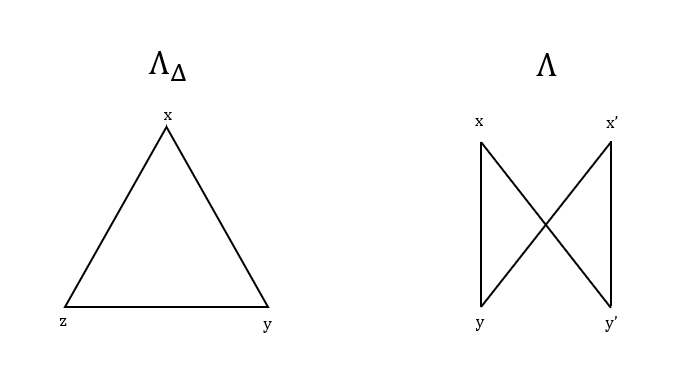
\includegraphics[scale=0.4]{GraphEntanglement.png}
\end{center}
\pause
We note that boundedness of the triangular Hilbert transform implies boundedness of the two dimensional bilinear Hilbert transform in some cases, so any improved understanding of entanglement is helpful.
\end{frame}



\begin{frame}
\frametitle{Ergodic averages}

Let $X$ be a probability space and let $T, S: X \to X$ be commuting measure-preserving transformations on $X$. For $f,g \in L^\infty(X)$, one can investigate the almost everywhere convergence of the averages
%
\begin{equation*}
\dfrac{1}{N}\sum\limits_{n=1}^{N}f(T^n x)g(S^{-n} x) \quad\text{as $N \to \infty$.}
\end{equation*}
%
\pause
Using a paraproduct estimate, Demeter and Thiele showed convergence of a related family of averages, including
%
\begin{equation}\label{jdjfergodic2}
\dfrac{1}{N^2}\sum\limits_{n=1}^{N}\sum\limits_{m=1}^{N}f(T^nS^m x)g(T^{-n}S^m x)
\end{equation}
\end{frame}

\begin{frame}
\frametitle{Bounding oscillation of ergodic averages}
What is one way to prove convergence of averages like those above?
\pause

Idea: attempt to bound (a weighted) version of the oscillation of the terms in a manner that essentially only depends on the $L^2$ norms of $f$ and $g$. If done correctly, we will obtain a.e. convergence of the average. \pause For instance, Demeter shows
\begin{equation*}
\begin{aligned}
    &\Big\| \Big(\sum \limits_{j=1}^{J-1}\sup_{k \in [u_j,u_{j+1})}\vert W_k(f, g)(x) - W_{u_{j+1}}(f, g)(x)\vert^2\Big)^{\frac{1}{2}} \Big\|_{L^{1, \infty}(X)}\\
    &\quad\quad\quad\quad\quad\quad\quad\quad\quad\quad\quad\quad\lesssim J^{\frac{1}{4}}\lVert f\rVert_{L^2(X)} \lVert g\rVert_{L^2(X)},
\end{aligned}
\end{equation*}
(where $W$ is the weighted average and $J$ is a term related to the oscillation) implies a.e. convergence.
\end{frame}


\begin{frame}
\frametitle{Transfer principle}
These kinds of bounds connect back to harmonic analysis via a transfer principle. The basic idea is as follows:\pause
\begin{itemize}
\item Consider functions on $\mathbb{R}^2$ which are constant on all the integer lattice squares $(n, n+1)\times(m, m+1)$; these are more-or-less functions on $\mathbb{Z}^2$. So, a bound obtained through harmonic analysis can give as a bound on such functions. \pause
\item Next, move from $\mathbb{Z}^2$ to the probability space $X$ by using the functions $F$ on $\mathbb{Z}^2$ which are of the form $F(n, m)=f(T^n S^mx)$ for some $x\in X$. \pause
\end{itemize}
Using this transfer principle, for instance, it suffices to prove an inequality for the oscillation of
\begin{equation*}
    \int_{\mathbb{R}^2} F_1(x + t, y + s) F_2(x -t, y+s) \Psi_k(t)\Phi_k(t) dtds
\end{equation*}
to obtain convergence of the second ergodic average.

\end{frame}


\begin{frame}
\frametitle{Key tools in proving the main theorem}
The proof of the main theorem proceeds first through a decomposition of the symbol into suitable pieces which we attempt to bound uniformly. These pieces are highly symmetric, and we can use a combination of Cauchy-Schwarz an a certain `telescoping identity' to gradually detangle the form.
\vspace{2mm}
\pause
Specifically, we have the following key tools:
\begin{enumerate}
    \item[(A)] A miniature version of time-frequency analysis, i.e. simultaneous decompositions of functions to localize behaviour in space and frequency.
\pause

    \item[(B)] Exploiting cancellation using the aforementioned telescoping identity, which for intuition's sake behaves like a multilinear variant of an integration by parts.
\pause

    \item[(C)] Using monotonicity to replacing arbitrary functions with concrete functions (e.g. Gaussians).
\end{enumerate}

\end{frame}

\begin{frame}
\frametitle{Decomposing the symbol I}

First, assume that $m(\xi, \eta)$ is supported on the double cone $\Gamma = \{ (\xi,\eta): |\xi| \leq 1.001 |\eta| \}$. If not, this can be handled with a smooth partition of unity.
\pause
\begin{center}
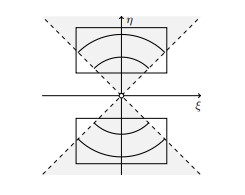
\includegraphics[scale=0.6]{MultiplierCone.jpg}
\end{center}
\pause
We define $\theta$ to be such that $\hat{\theta}$ is smooth, real, radial, and supported in some annulus. Normalizing $\hat{\theta}$ and defining $m_t(\xi, \eta):=m(\xi,\eta)\hat{\theta}(t\xi,t\eta)$ allows us to write
\begin{equation*}
    m(\xi, \eta) =\int_0^\infty m_t(\xi, \eta)\dfrac{dt}{t}.
\end{equation*}
\end{frame}

\begin{frame}
\frametitle{Decomposing the symbol II}
Using a technical lemma, we obtain the existence of sufficiently nice functions $\nu_1, \nu_2$ that satisfy
\begin{equation*}
    m_t(\xi, \nu)= m_t(\xi, \nu)\hat{\nu}_1(t\xi)\hat{\nu}_2(t\eta)
\end{equation*}
\pause
Using Fourier inversion, we obtain
\begin{equation*}
m_t(\xi, \eta)=\left(\int_{\mathbb{R}^2}\mu_t(u, v) e^{2\pi i u t \xi}e^{2\pi i v t \eta}\right)\hat{\nu}_1(t\xi)\hat{\nu}_2(t\eta)
\end{equation*}
with $\mu_t(u, v):=t^2\hat{m}(tu, tv)$.\pause It is not hard to show that
\begin{equation*}
\vert \mu_t(u, v)\vert \lesssim (1+\vert u\vert)^{-12} (1+\vert v\vert)^{-12}
\end{equation*}

\end{frame}

\begin{frame}
\frametitle{Decomposing the symbol III}
Now, define
\begin{equation*}
\widehat{\varphi}_{t,u}(\xi):=(1+\vert u \vert)^{-5} \hat{\nu}_1(t\xi)^{1/2}e^{\pi i u t\xi}
\end{equation*}
\begin{equation*}
\widehat{\psi}_{t,v}(\xi):= \hat{\nu}_2(t\xi)^{1/2}e^{\pi i v t\eta}
\end{equation*}
\pause
Using the properties of the $\nu_i$, we have,
\begin{equation*}
m(\xi, \eta) = \int \mu_t(u, v)(1+\vert u \vert)^{10}\widehat{\varphi}_{t,u}(\xi)^2 \widehat{\psi}_{t,v}(\xi)^2\; du dv \dfrac{dt}{t}
\end{equation*}
\pause
Note that $\mu_t(u, v)(1+\vert u \vert)^{10}$ decays rapidly. So, it suffices to establish bounds on
\begin{equation*}
\int \widehat{\varphi}_{t,u}(\xi)^2 \widehat{\psi}_{t,v}(\xi)^2\; \widehat{\mathbf{F}}(\xi,-\xi,\eta,-\eta)\; \dfrac{dt}{t} d\xi d\eta
\end{equation*}
uniformly in $u$ and $v$.
\end{frame}






\begin{frame}
    \frametitle{The Setup}

    % Write Definition of F on the blackboard

    \begin{goal}
        \small

        \vspace{-1em}
        \[ \text{Show}\quad \left| \int \widehat{\mathbf{F}}(\xi,-\xi,\eta,-\eta) \widehat{\varphi}_t(\xi)^2 \widehat{\psi}_t(\xi)^2\; (dt/t)\; d\xi\; d\eta \right| \lesssim 1. \]
    \end{goal}

    % Kind of like singular integral, e.g. the Hilbert transform, where we'd obtain bounds for the transform given uniform bounds in t above.

    % At this point, draw pictures of the functions varphi and psi, and also their reflections?

    \pause

    \begin{singular}
        \small

        Bound above is equivalent to $|\int_0^\infty \Lambda_t\; dt/t| \lesssim 1$, where
        \vspace{-0.5em}
        \[ \Lambda_t = \int \mathbf{F}(x,y,x',y') \varphi_t(\tilde{x} - x) \varphi_t^-(\tilde{x} - x') \psi_t(\tilde{y} - y) \psi_t^-(\tilde{y} - y'). \]
    \end{singular}

    \pause

    \begin{notation}
        \small
        Write $\Lambda_t = \Lambda_{\varphi_t, \varphi_t^-, \psi_t, \psi_t^-}$, where
        %
        \vspace{-0.5em}
        \[ \Lambda_{a,b,c,d} = \int \mathbf{F}(x,y,x',y') a(\tilde{x} - x) b(\tilde{x} - x') c(\tilde{y} - y) d(\tilde{y} - y'). \]
    \end{notation}
    
    % Average in each variable, but *entangled average*.
\end{frame}

\begin{frame}
    \frametitle{Disentangling with Cauchy-Schwarz}

    \small

    \begin{collectyvariables}
    %
    \vspace{-0.8em}
    \begin{align*}
        \Lambda_t &= \int F_1(x,y) F_2(x',y) F_3(x',y') F_4(x,y')\\
        &\quad\quad\quad \varphi_t(\tilde{x} - x) \varphi_t^-(\tilde{x} - x')\; \psi_t(\tilde{y} - y) \psi_t^-(\tilde{y} - y')\\
        &= \int \left( \int F_1(x,y) F_2(x',y) \psi_t(\tilde{y} - y)\; dy \right)\\
        &\quad\quad\quad \left( \int F_4(x,y') F_3(x',y') \psi_t^-(\tilde{y} - y')\; dy' \right)\\
        &\quad\quad\quad\quad\quad \varphi_t(\tilde{x} - x) \varphi_t^-(\tilde{x} - x')\; dx\; dx'\; d\tilde{x}\; d\tilde{y}.
    \end{align*}

    \end{collectyvariables}

    \pause

    \begin{remark}
        Cauchy-Schwarz is efficient (All $F_j$ are equal in the worst case).
    \end{remark}
\end{frame}

\begin{frame}

    \begin{cauchyschwarz}
        \footnotesize

        \[ \left| \int A B C D \right| \leq \left( \int A A |C| \right)^{\frac{1}{2}} \left( \int B B |D| \right)^{\frac{1}{2}}. \]
        %

        \pause

        Set
        %
        \[ A = \int F_1(x,y) F_2(x',y) \psi_t(\tilde{y} - y)\; dy \]
        %
        \[ B = \int F_4(x,y') F_3(x',y') \psi_t(\tilde{y} - y')\; dy' \]
        %
        and
        %
        \[ C = \varphi_t(\tilde{x} - x) \quad\quad D = \varphi_t^-(\tilde{x} - x'). \]
    \end{cauchyschwarz}
    %

    \pause
    
    \begin{result}
        \footnotesize

        Since $\Lambda_t = \int A B C D$, we obtain that
        %
        \vspace{-0.8em}
        \begin{align*}
            |\Lambda_t| &\leq \Lambda_{|\varphi_t|, |\varphi_t^-|, \psi_t, \psi_t}(F_1,F_2,F_2,F_1)^{1/2}\\
            &\quad\quad \Lambda_{|\varphi_t|, |\varphi_t^-|, \psi_t^-, \psi_t^-}(F_4,F_3,F_3,F_4)^{1/2}.
        \end{align*}
    \end{result}
\end{frame}

%\begin{frame}
%    \frametitle{Expanding Out Squares}

%    \begin{expandoutsquares}
%        \footnotesize
%        Note that
%        %
%        \begin{align*}
%            &\int \left| \int F_1(x,y) F_2(x',y) \psi_t(\tilde{y} - y)\; dy \right|^2 |\varphi_t(\tilde{x} - x)| |\varphi_t^-(\tilde{x} - x')|\\
%            &\quad = \int F_1(x,y) F_2(x',y) F_1(x,y') F_2(x',y')\\
%            &\quad\quad\quad\quad |\varphi_t(\tilde{x} - x)| |\varphi_t^-(\tilde{x} - x')| \psi_t(\tilde{y} - y) \psi_t^-(\tilde{y} - y')\\
%            &\quad = \Lambda_{|\varphi_t|, |\varphi_t^-|, \psi_t, \psi_t^-}(F_1,F_2,F_2,F_1)
%        \end{align*}
        %
%        Thus we've shown
        %
%        \[ |\Lambda_t| \leq \Lambda_{|\varphi_t|, |\varphi_t^-|, \psi_t, \psi_t^-}(F_1,F_2,F_2,F_1)^{1/2}\; \Lambda_{|\varphi_t|, |\varphi_t^-|, \psi_t, \psi_t^-}(F_3,F_4,F_4,F_3)^{1/2}. \]
%    \end{expandoutsquares}
%\end{frame}

\begin{frame}
    \frametitle{Multilinear Integration By Parts}

    \begin{remark}
        Want to do the same trick with the $x$ and $x'$ variables, but we can't without losing cancellation since we'd have to take absolute values of $\psi_t$ and $\psi_t^-$. Can `juggle' the cancellation by integrating by parts in $t$.
    \end{remark}

    \pause

    \begin{ibpidentity}
        If $-t \partial_t | \widehat{\rho}_i |^2 = |\widehat{\sigma}_i(t \tau)|^2$, then
        %
        \begin{align*}
            \int \Lambda_{\sigma_1, \sigma_1, \rho_2, \rho_2}\; (dt / t) &= - \int \Lambda_{\rho_1, \rho_1, \sigma_2, \sigma_2}\; (dt / t).\\
            &\quad\quad\quad + |\widehat{\rho}_1(0)|^2 |\widehat{\rho}_2(0)|^2 \int_{\RR^2} F_1 F_2 F_3 F_4
        \end{align*}
    \end{ibpidentity}
\end{frame}

\begin{frame}
    \frametitle{Examples of Pairs of $\rho$ and $\sigma$}

    Example Pairs are given by
    %
    \[ \rho(t,x) = t^{-1} e^{-(x/t)^2} \quad\text{and}\quad \sigma(t,x) = - (4 \pi^{1/2} x / t^2) e^{-2 \pi (x/t)^2}. \]
    %
    \begin{center}
    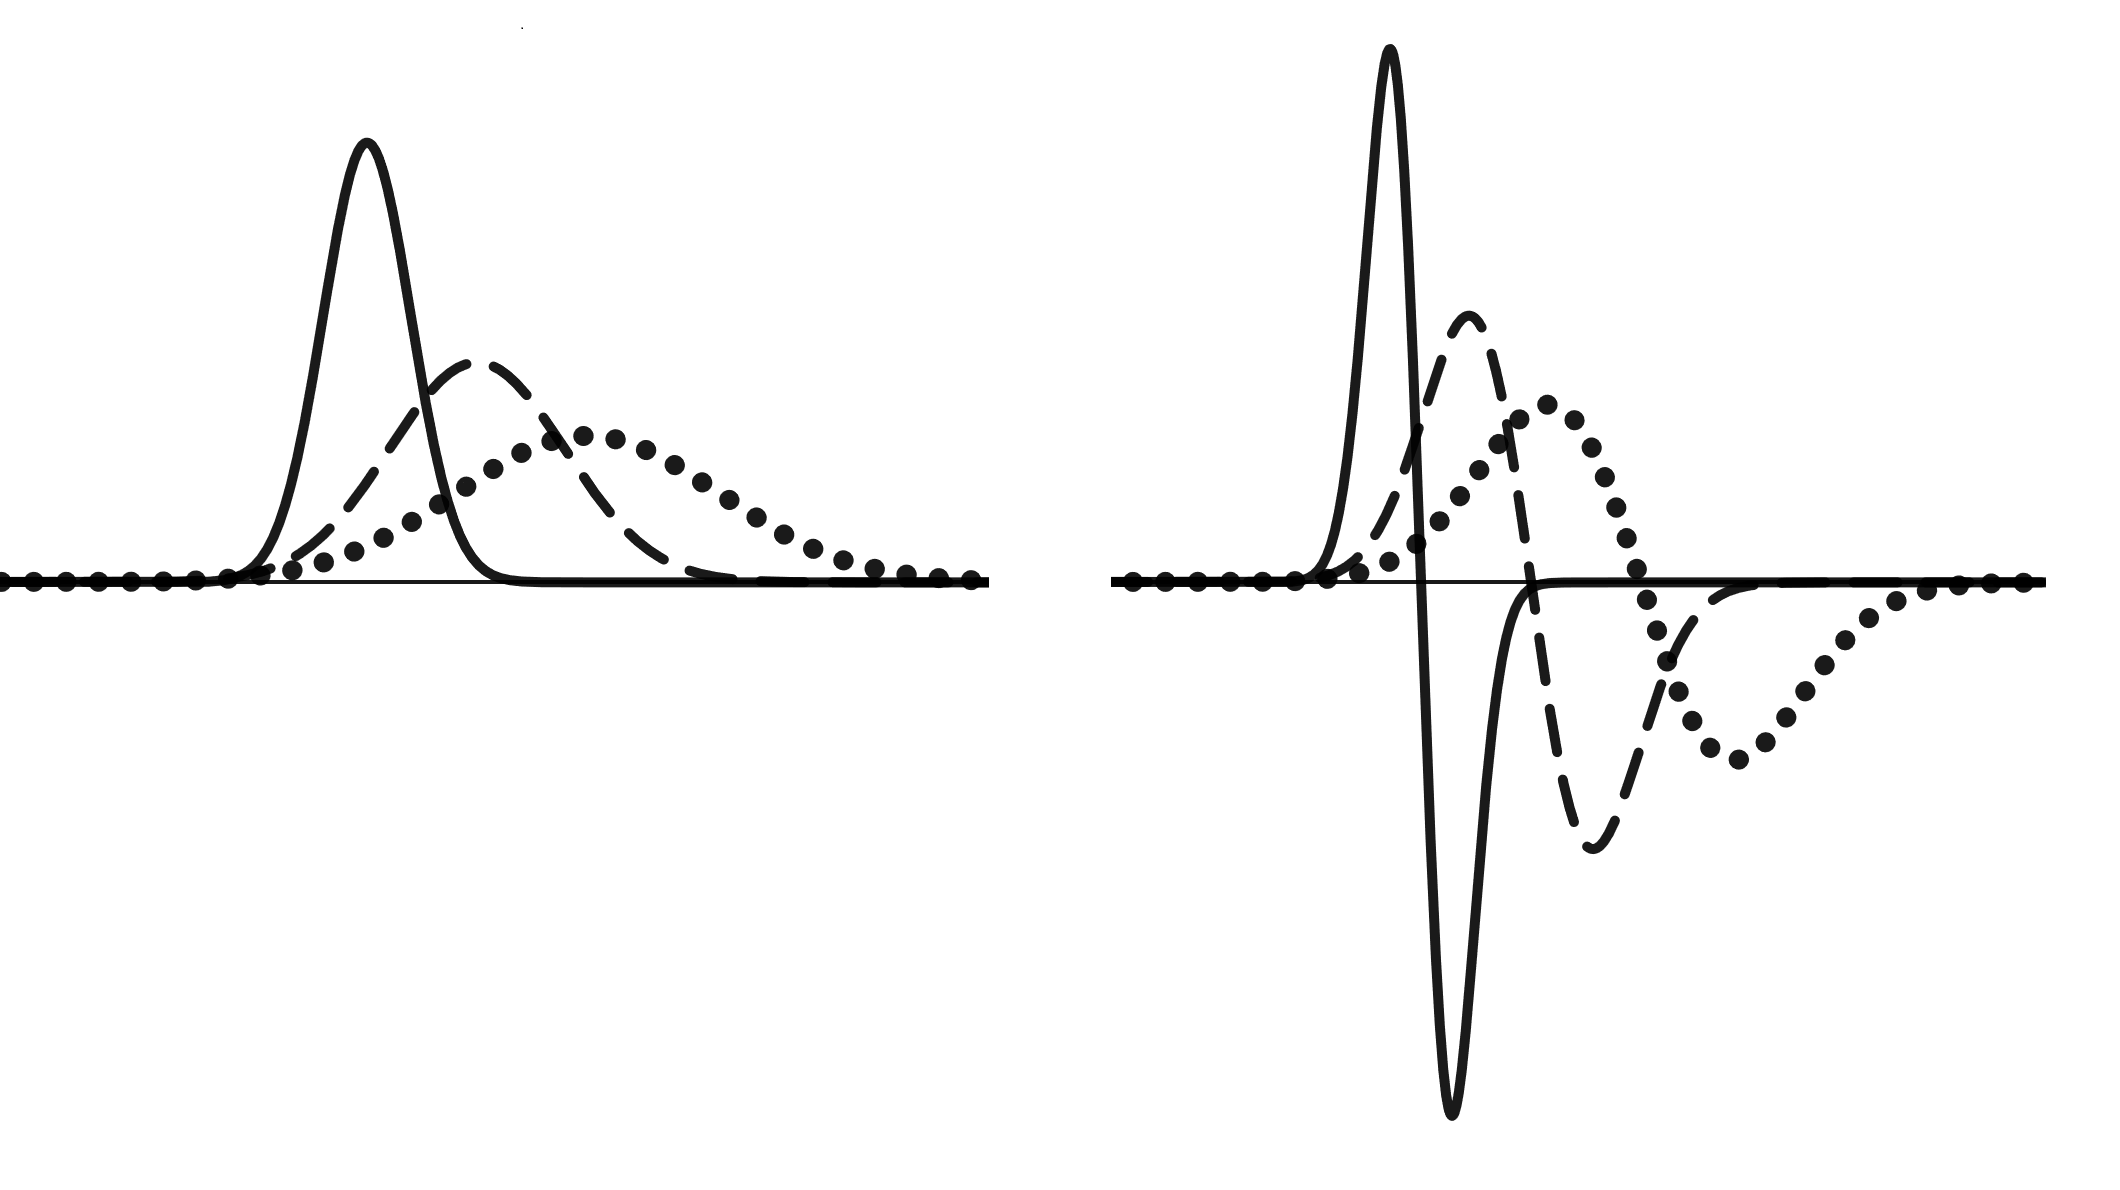
\includegraphics[scale=0.2]{JDJFrhoandsigma.png}
    \end{center}
\end{frame}

\begin{frame}
    \begin{proofofidentity}
    Write
    %
    \vspace{-0.5em}
    \begin{align*}
        - |\widehat{\rho}_1(0)|^2 |\widehat{\rho}_2(0)|^2 &= \int_0^\infty \partial_t \{ |\widehat{\rho}_1(t \xi)|^2 |\widehat{\rho}_2(t \eta)|^2 \}\; dt\\
        &= \int_0^\infty t \partial_t \{ |\widehat{\rho}_1(t \xi)|^2 \} |\widehat{\rho}_2(t \eta)|^2\; (dt / t)\\
        &\quad + \int_0^\infty |\widehat{\rho}_1(t \xi)|^2 t \partial_t \{ |\widehat{\rho}_2(t \eta)|^2\; (dt / t).
    \end{align*}
    %
    Now multiply by $\widehat{\mathbf{F}}(\xi, -\xi, \eta, - \eta)$, and integrate in $\xi$ and $\eta$.
    \end{proofofidentity}
\end{frame}

\begin{frame}
    \frametitle{Using the Identity}

    \begin{ibpidentity}
        If $-t \partial_t | \widehat{\rho}_i |^2 = |\widehat{\sigma}_i(t \tau)|^2$, then
        %
        \begin{align*}
            \int \Lambda_{\sigma_1, \sigma_1, \rho_2, \rho_2}\; (dt / t) &= - \int \Lambda_{\rho_1, \rho_1, \sigma_2, \sigma_2}\; (dt / t).\\
            &\quad\quad\quad + |\widehat{\rho}_1(0)|^2 |\widehat{\rho}_2(0)|^2 \int_{\RR^2} F_1 F_2 F_3 F_4
        \end{align*}
    \end{ibpidentity}

    \begin{problems}
        We cannot use this to directly bound
        %
        \vspace{-0.7em}
        \[ |\Lambda_{|\varphi_t|, |\varphi_t^-|, \psi_t, \psi_t}(F_1,F_2,F_2,F_1)|. \]
    \end{problems}
\end{frame}

\begin{frame}
    \frametitle{Monotonicity}

    \begin{monotonicity}

    We have
    %
    \vspace{-0.8em}
    \begin{align*}
        \Lambda_{a,a',b,b} &= \int \left( \int F_1(x,y) F_2(x',y) b(\tilde{y} - y)\; dy \right)^2\\
        &\quad\quad\quad\quad\quad\quad a(\tilde{x} - x) a'(\tilde{x} - x'),
    \end{align*}
    %
    and so $\Lambda_{a,a',b,b}$ is  \emph{monotonic} in $a$ and $a'$.

    \end{monotonicity}

    \pause

    \begin{replacingfunctionswithgaussians}
    Let $G_{t,\alpha} = \alpha^{-1} \exp(-(x/\alpha)^2)$ be normalized Gaussians. For appropriate fast decaying constants $C$ and $C'$,
    %
    \small

    \vspace{-1em}
    \[ |\varphi_t| + |\varphi_t^-| \leq |\varphi_t| + |\varphi_t^-| \leq \int_1^\infty C(\alpha) G_{t,\alpha}. \]
    %
    \vspace{-1.2em}
    \[ \text{Thus}\quad \Lambda_{|\varphi_t|,|\varphi_t^-|,\psi_t, \psi_t} \leq \int_1^\infty C'(\alpha) \Lambda_{G_{t,\alpha}, G_{t,\alpha}, \psi_t, \psi_t}. \]
    %
    It suffices to prove uniform estimates in $\alpha$.
    \end{replacingfunctionswithgaussians}
\end{frame}

\begin{frame}
    \frametitle{Back to Cauchy Schwarz}

    \begin{ApplyIBP}
    \[ \Lambda_{G_t, G_t, \psi_t, \psi_t} = c \int F_1^2 F_2^2 - \Lambda_{g_t,g_t, \Psi_t, \Psi_t}. \]
    %
    Notice that the oscillating term has been moved to the third and fourth term.
    \end{ApplyIBP}

    \pause

    \begin{cauchyschwarz}
    We can now use Cauchy-Schwarz while preserving oscillation.
    %
    \begin{align*}
        &\Lambda_{g_t,g_t, \Psi_t, \Psi_t}(F_1,F_2,F_2,F_1)\\
        &\quad\quad \leq \Lambda_{g_t,g_t,|\Psi_t|, |\Psi_t|}(F_1,F_1,F_1,F_1)^{1/2}\\
        &\quad\quad\quad\quad\quad \Lambda_{g_t,g_t,|\Psi_t|, |\Psi_t|}(F_2,F_2,F_2,F_2)^{1/2}.
    \end{align*}
    \end{cauchyschwarz}
\end{frame}





\begin{frame}
    \frametitle{A Final Integration By Parts}

    \begin{monotonicity}
    Use monotonicity to switch the $\Psi_t$ values with a Gaussian, i.e. so that
    %
    \vspace{-0.7em}
    \[ \Lambda_{g_t,g_t,|\Psi_t|, |\Psi_t|}(F_1,F_1,F_1,F_1) \lesssim \Lambda_{g_t,g_t,G_t', G_t'}(F_1,F_1,F_1,F_1). \]
    \end{monotonicity}

    \pause

    \begin{ApplyIBP}

    We can now perform a final integration by parts to write
    %
    \vspace{-0.5em}
    \[ \Lambda_{g_t,g_t,G_t', G_t'}(F_1,F_1,F_1,F_1) = c \int F_1^4 - \Lambda_{G_t,G_t,g_t',g_t'}(F_1,F_1,F_1,F_1). \]
    %
    But both the $\Lambda$ terms here are \emph{positive}, i.e. they cannot cancel one another out.
    %
    \vspace{-0.5em}
    \[ \Lambda_{g_t,g_t,G_t', G_t'}(F_1,F_1,F_1,F_1) \lesssim \int F_1^4 = \| F_1 \|_{L^4(\RR^2)}^4. \]
    \end{ApplyIBP}
\end{frame}

\end{document}